\documentclass{llncs}
\usepackage{enumerate}
\usepackage{caption}
\usepackage{graphicx}
	 
\title{CSE 501: Implementation of Programming Languages\\ Programming Assignment 1}
\author{Haichen Shen}
\institute{}

\begin{document}

\maketitle

\section{Description: CFG Construction and Dominators}
The goal is to construct the control flow graph for each method and then find the immediat dominator for each basic block.

\section{Implementation}
Inside this project, I use the algorithm created by Cooper, Harvey and Kennedy to find the immediate dominators. The main idea of this method is finding the closest common immdiate dominator of all predecessors of one node.

Main flow of my program is:
\begin{enumerate}
	\item Read the whole start file, parse the routines inside this file and create a class {\it Routine} for each routine.
	\item For every routine, find the basic blocks inside the method, create a class {\it BasicBlock} for each basic block, and generate the CFG.
	\item Now iterate each routine and run the idom algorithm:
	\begin{enumerate}[3a.]
		\item Generate postorder sequence of all block.
		\item According to inverse postorder, iteratively update the idom for each block.
	\end{enumerate}
\end{enumerate}

The project is implemented in Java.

\section{Measurements}
I measured the time consumption in two parts respectively: (i) finding the basic and building CFG, (ii) finding dominators. I ran 10 times for a program and use the average time as the result. Firstly, I ran the tests on all example programs. The result is shown in Table \ref{tab:test1}.

\begin{table}[h]
\centering
\begin{tabular}{|c|c|c|c|c|}
\hline
Program & Build the CFG($\mu$s) & Find dominators($\mu$s) & Total basic block & Max basic block in a routine \\\hline
points & 2538.36 & 403.39 & 8 & 4
\\\hline
mmm & 4247.37 & 942.76 & 44 & 40
\\\hline
cd & 2437.39 & 363.11 & 5 & 4
\\\hline
hanoifibfac & 2836.37 & 490.58 & 15 & 4
\\\hline
rime & 2746.81 & 500.03 & 13 & 13
\\\hline
rational & 3545.57 & 569.73 & 19 & 9
\\\hline
truct & 3159.37 & 421.92 & 7 & 7
\\\hline
ieve & 2794.85 & 524.84 & 16 & 16
\\\hline
link & 2540.44 & 411.33 & 9 & 4
\\\hline
oop & 2755.69 & 584.24 & 19 & 19
\\\hline
lass & 2486.10 & 365.65 & 5 & 3
\\\hline
sort & 2904.28 & 559.56 & 18 & 18
\\\hline
regslarge & 14727.42 & 354.22 & 4 & 4
\\\hline
\end{tabular}
\caption{Time consumption in building CFG and finding dominators}
\label{tab:test1}
\end{table}

I think the reason that it take quite a long time to build the control flow graph is because (i) firstly it takes some time to go through the all instructions the find out all basic blocks and go through the blocks again to build the control flow graph; (ii) I also copy the instructions to each block and it could slow down the program.

Besides I notice that the time in finding dominatros are related to the max basic blocks in a routine. But it is uncertain what kind of relationship they are. 

Therefore I write a small program which generatee loop program to figure out the relationship between the block numbers and time consumption in finding idom. The name of prgroam means how many layers of loop inside. And every test program has only the main function. The result of the my testing programs shows in Table \ref{tab:test2}.

\begin{table}[h]
\centering
\begin{tabular}{|c|c|c|c|c|}
\hline
Program & Find dominators($\mu$s) & Basic blocks \\\hline
loop20 & 1178.58 & 61 
\\\hline
loop40 & 1971.86 & 121
\\\hline
loop80 & 3501.38 & 241
\\\hline
loop100 & 4287.60 & 301
\\\hline
loop200 & 8536.69 & 601 
\\\hline
loop400 & 15903.11 & 1201
\\\hline
loop800 & 32763.57 & 2401 
\\\hline
\end{tabular}
\caption{Time consumption test}
\label{tab:test2}
\end{table}

In the Figure \ref{fig:1}, it is apparent that the time grows linearly along with the number of basic blocks which means that the complexity of algorithm should be $O(n)$. I haven't tried other programs. Since the loop program is quite simple and doesn't have a complex CFG, probably it's only for the simple program that the time consumption is linear to number of blocks.

\begin{figure}[h]
\centering
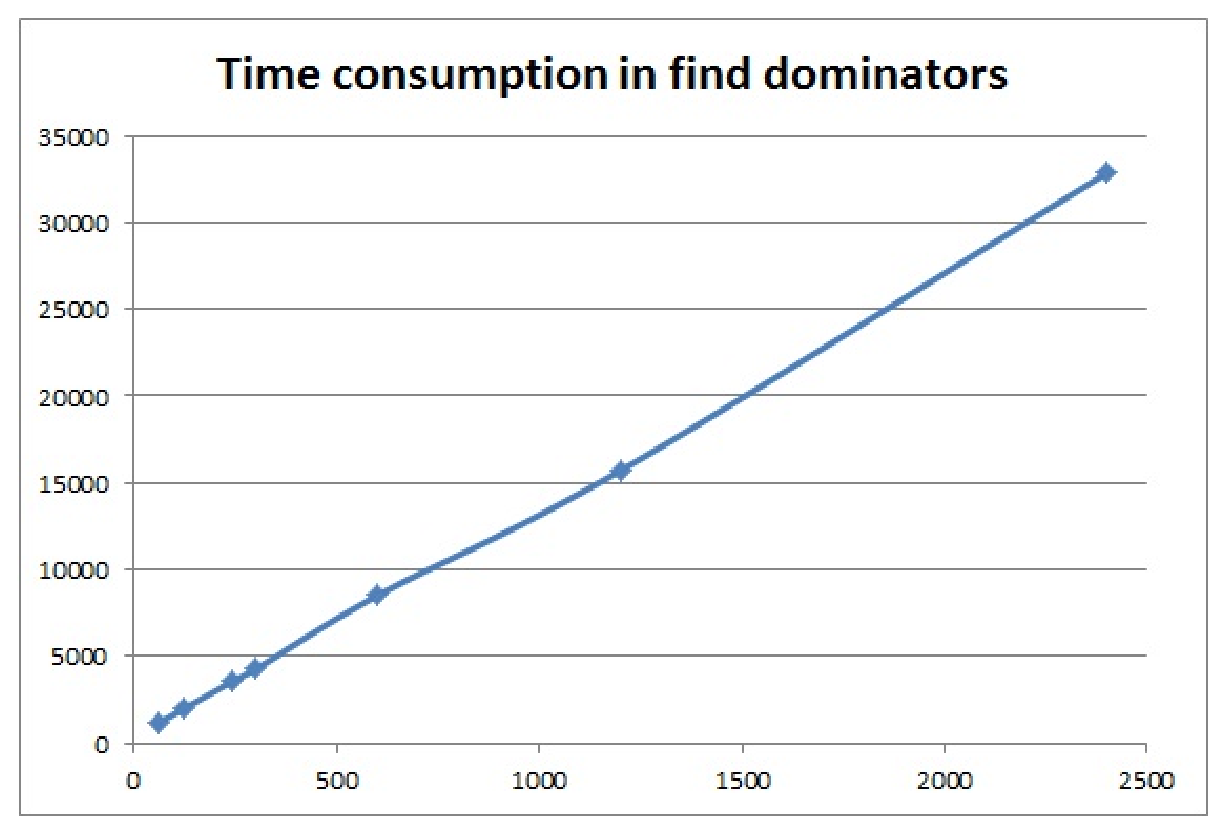
\includegraphics[height=7.5cm]{fig.eps}
\caption{Relationship between block number and time consumption. X-axis: the number of basic blocks, Y-axis: the time consumption ($\mu$s)}
\label{fig:1}
\end{figure}

%\bibliographystyle{abbrv}
%\bibliography{ref}

\end{document}
